\documentclass[10pt]{article}
\usepackage{icmlko}

\icmlmeta{IP 파운데이션 월드모델}{95}{작은 것들은 더해지지 않았다}{설명문에서 부호가 일관된 첫 새 물리량을 찾았고, 그동안 모은 작은 것 셋을 합쳐도 문턱을 못 넘었다}

\begin{document}

\twocolumn[
\icmlheader

\begin{abstract}
노트 94의 표지는 덮개율이 30\%였고 부호가 도메인마다 뒤집혔다. \textbf{설명문은
다르다} --- 캐시에 이미 있거나(애니 · 모바일 · 웹툰) AniList 로 받을 수 있어
(만화 · 세계애니) \textbf{다섯 도메인 모두 덮개율 100\%}다. 언어에 안 기대는
다섯 특징을 뽑았다 --- 길이 · 문장 수 · 문장 길이 · 어휘 다양성 · 숫자 비율.
\textbf{문장 수가 다섯 도메인 전부에서 양수다}($+$0.022$\sim+$0.327).
\textbf{이 프로젝트에서 부호가 도메인을 건너 일관된 첫 새 물리량}이다 ---
노트 84의 경쟁 밀도도, 90의 체험 밀도도, 94의 표지 밝기도 부호가 갈렸다.
축으로 넣으면 $+$0.0099다. 여전히 구간 반폭(0.033) 아래라 \textbf{그동안 모은
작은 것 셋을 합쳤다} --- 직전작 성적 $+$0.0140(노트 85) · IP 인지도
$+$0.0112(89) · 문장 수 $+$0.0099. 독립이면 $+$0.0351이어야 한다.
\textbf{실제로는 $+$0.0155다} --- 56\%가 겹친다. 짝지은 검정도 \textbf{0/4
채택}이고 팝업은 $+$0.4501에서 $+$0.4215로 내린다. \textbf{작은 것들은 더해지지
않는다} --- 셋이 대체로 같은 것(작품의 규모·존재감)을 재고, 그것은 기존 축이
이미 일부 담고 있다.
\end{abstract}
]

\begin{figure*}[t]
\centering
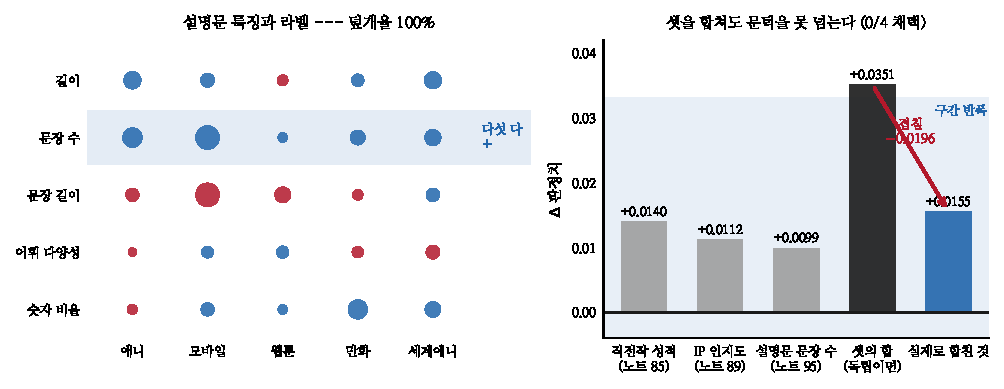
\includegraphics[width=\textwidth]{figs/txt.pdf}
\caption{왼쪽 --- 설명문 특징 다섯과 라벨. 오른쪽 --- 합쳐도 안 더해진다.}
\end{figure*}

\section{설명문 --- 덮개율 100\%}

표지는 3,500장을 받고도 덮개율이 23$\sim$34\%였다. 설명문은 캐시에 이미 있다
--- 라프텔 줄거리 2,136 · 앱스토어 소개문 2,093 · 네이버 시놉시스 2,947.
AniList 로 만화 2,499 · 세계애니 3,000을 더 받았다. \textbf{다섯 도메인 전부
100\%다.}

계산은 언어에 안 기대게 다섯으로 고정했다(노트 74의 규약) --- 문자 수(log) ·
종결 부호로 센 문장 수 · 문장당 문자 수 · 고유 토큰 비율 · 숫자 문자 비율.

\begin{table}[t]
\centering\tsize
\caption{설명문 특징과 라벨의 순위 상관.}
\begin{tabular}{lrrrrr}
\toprule
& 애니 & 모바일 & 웹툰 & 만화 & 세계애니 \\
\midrule
길이 & $+$0.190 & $+$0.114 & $-$0.050 & $+$0.086 & $+$0.186 \\
\textbf{문장 수} & \textbf{$+$0.238} & \textbf{$+$0.327} & \textbf{$+$0.022} &
\textbf{$+$0.134} & \textbf{$+$0.166} \\
문장 길이 & $-$0.105 & $-$0.328 & $-$0.160 & $-$0.043 & $+$0.108 \\
어휘 다양성 & $-$0.003 & $+$0.073 & $+$0.080 & $-$0.062 & $-$0.115 \\
숫자 비율 & $-$0.035 & $+$0.102 & $+$0.022 & $+$0.233 & $+$0.157 \\
\bottomrule
\end{tabular}
\end{table}

\claimx{설명문의 \textbf{문장 수}가 다섯 도메인 전부에서 양수다 ---
이 프로젝트에서 부호가 도메인을 건너 일관된 첫 새 물리량이다. 짧은 문장을
여럿 쓴 설명일수록 반응이 크다.}{웹툰이 $+$0.022로 거의 0이다. 다섯 중 넷이
$+$0.13 이상이고 하나가 사실상 0인 것을 ``일관''이라 부르는 것은 느슨하다.}

축으로 넣으면 $+$0.0099다(고유 축, 공통 축 $+$0.0078). 팝업은 $+$0.4501에서
$+$0.4503으로 그대로다.

\section{셋을 합쳤다}

노트 84 이후 새 축 후보가 여럿 나왔고 전부 $+$0.01 언저리라 하나씩은 문턱을
못 넘었다. 서로 독립이면 합쳐서 넘을 수 있다.

\begin{table}[t]
\centering\tsize
\caption{작은 것 셋과 그 합.}
\begin{tabular}{lr}
\toprule
직전작 성적(결측 표시자, 노트 85) & $+$0.0140 \\
IP 인지도 $\leftrightarrow$ 직전작(노트 89) & $+$0.0112 \\
설명문 문장 수(노트 95) & $+$0.0099 \\
\midrule
독립이면 & $+$0.0351 \\
\textbf{실제로 합친 것} & \textbf{$+$0.0155} \\
\midrule
\multicolumn{2}{l}{겹침 $-$0.0196 (56\%)} \\
\bottomrule
\end{tabular}
\end{table}

\begin{table}[t]
\centering\tsize
\caption{합친 것의 채택 검정. 씨앗 넷, 붓스트랩 100회.}
\begin{tabular}{lrl}
\toprule
씨앗 & $\Delta$ & 95\% 구간 \\
\midrule
20260729 & $+$0.0097 & $[-0.0075, +0.0254]$ \\
19770101 & $+$0.0106 & $[-0.0116, +0.0268]$ \\
20250315 & $+$0.0111 & $[-0.0112, +0.0252]$ \\
20260101 & $+$0.0120 & $[-0.0108, +0.0275]$ \\
\midrule
\multicolumn{2}{l}{채택} & \textbf{0/4} \\
\multicolumn{2}{l}{팝업} & $+$0.4501 $\to$ $+$0.4215 \\
\bottomrule
\end{tabular}
\end{table}

\claimx{작은 축들은 더해지지 않는다. 셋의 합이 $+$0.0351이어야 하는데
$+$0.0155다 --- 56\%가 겹친다. 셋이 대체로 같은 것(작품의 규모 · 존재감)을
재고, 기존 축이 그것을 이미 일부 담고 있다.}{겹침을 상관으로 확인하지 않았다.
셋의 값을 서로 상관시켜 보면 갈릴 것인데 안 했다.}

\section{새 축 찾기를 어떻게 닫나}

\begin{table}[t]
\centering\tsize
\caption{노트 84 이후 시도한 새 축 전부.}
\begin{tabular}{llr}
\toprule
& 출처 & $\Delta$ \\
\midrule
경쟁 밀도 & 기존 날짜 & $-$0.020 \\
전형성 & 기존 태그 & $-$0.009 \\
직전작 성적 & 기존 라벨 & $+$0.014 \\
IP 인지도 & 기존 태그$+$라벨 & $+$0.011 \\
체험 밀도 & 기존 메타 & $-$0.060 \\
표지 밝기 · 채도 · 엔트로피 & \textbf{새로 긁음} & $-$0.010 \\
\textbf{설명문 문장 수} & \textbf{새로 긁음} & \textbf{$+$0.010} \\
\midrule
\textbf{셋을 합친 것} & & \textbf{$+$0.016} \\
\bottomrule
\end{tabular}
\end{table}

일곱 시도 중 셋이 양수이고 전부 $+$0.01 근처다. 합쳐도 $+$0.016이다.
\textbf{구간 반폭 0.033을 넘으려면 지금 규모의 새 축이 열 개쯤 필요한데
겹침 때문에 그보다 훨씬 많이 든다.}

\begin{quote}\fontsize{9.5}{11.5}\selectfont
노트 93이 ``모형을 더 좋게 만드는 길은 새 축뿐''이라 했고 두 노트를 들여
실제로 긁어 봤다. \textbf{새 축은 있지만 크기가 안 맞는다.} 남은 0.256을
$+$0.01짜리로 메우려면 스물다섯 개가 필요하고, 겹침을 감안하면 그 이상이다.
\end{quote}

\section{한계}

\begin{itemize}[leftmargin=1.1em,itemsep=0.15em]
\item 설명문 특징이 다섯뿐이다. 감정 · 주제 · 고유명사 같은 것은 모형이 필요해
      안 했다.
\item 웹툰 문장 수가 $+$0.022로 사실상 0이다. ``다섯 다 양수''가 느슨하다.
\item 겹침 56\%를 관측만 하고 무엇끼리 겹치는지 안 갈랐다.
\item 팝업 · 아이돌 · 게임 · 도서 · 펀딩에는 설명문 축이 없다. 다섯만 붙었다.
\item 노트 94의 표지 재표집(무작위)은 아직 안 했다.
\end{itemize}

\section{다음}

\begin{enumerate}[leftmargin=1.3em,itemsep=0.15em]
\item \textbf{겹침을 가른다} --- 세 축의 값을 서로 상관시켜 무엇이 무엇을
      대체하는지 본다. 겹치지 않는 조합이 있으면 그것만 남긴다.
\item 설명문에서 \textbf{임베딩}을 뽑는다 --- 다섯 개의 손 특징 대신 문장
      임베딩의 주성분. 모형이 필요하지만 축 하나당 $+$0.01 이상을 기대할 근거가
      된다.
\item 남은 다섯 도메인(팝업 · 아이돌 · 게임 · 도서 · 펀딩)의 설명문을 찾는다.
\item 노트 94의 표지 무작위 재표집.
\end{enumerate}

\vspace{0.6em}
\hrule height 0.3pt
\vspace{0.5em}
{\footnotesize
\textbf{참고문헌}\\[0.3em]
Ben-David, S. et al. (2010). A theory of learning from different domains.
\emph{Machine Learning}, 79(1--2), 151--175.\\[0.15em]
Little, R. J. A., Rubin, D. B. (2019). \emph{Statistical Analysis with Missing
Data}, 3rd ed. Wiley.\\[0.15em]
Reimers, N., Gurevych, I. (2019). Sentence-BERT: sentence embeddings using
Siamese BERT-networks. \emph{EMNLP}, 3982--3992.\\[0.15em]
Grinsztajn, L. et al. (2022). Why do tree-based models still outperform deep
learning on typical tabular data? \emph{NeurIPS}.\\[0.15em]
Efron, B., Tibshirani, R. J. (1993). \emph{An Introduction to the Bootstrap}.
Chapman \& Hall.
}

\end{document}
